\definecolor{cfwone}{HTML}{eef5fa}
\definecolor{cfwtwo}{HTML}{daeaf5}
\definecolor{cfwthree}{HTML}{b2d2e9}
\definecolor{cfwfour}{HTML}{8abbde}

\newcommand{\fwone}[1]{\colbox{cfwone}{#1}\xspace}
\newcommand{\fwtwo}[1]{\colbox{cfwtwo}{#1}\xspace}
\newcommand{\fwthree}[1]{\colbox{cfwthree}{#1}\xspace}
\newcommand{\fwfour}[1]{\colbox{cfwfour}{#1}\xspace}

\newcommand{\fexp}[2]{\texttt{[{\color{darkgray}{#1:#2}}]}\xspace}
\newcommand{\fexptag}[1]{\fexp{TAG}{#1}}
\newcommand{\fexpfrom}[1]{\fexp{FROM}{#1}}
\newcommand{\fexpto}[1]{\fexp{TO}{#1}}
\newcommand{\fexptemp}[1]{\fexp{TEMP}{#1}}


\section{Counterfactual Explanations}
\label{sec:app_explain}

\begin{figure}[t]
\centering
\includegraphics[trim={0 21cm 33cm 0cm},clip,width=1\columnwidth]{figures/explanation_v2.pdf}
\vspace{-15pt}
\caption{
(A) A \qqp instance with its prediction\footnotemark{} showing 98.2\% confidence that the two sentences are duplicates ($=$), as well as the SHAP weights.
%Counterfactual explanations complement SHAP with concrete, readable examples, \eg (C) depicts a surprising flipped prediction ($\neq)$ that was missed by SHAP.
Counterfactual explanations complement SHAP with concrete examples and flag abnormalities missed by SHAP, \eg (C)
depicts a surprising flipped prediction ($\neq)$.
}
\vspace{-10pt}
\label{fig:explanation}
\end{figure}

\footnotetext{From BERT \qqp model: \url{https://huggingface.co/textattack/bert-base-uncased-QQP}}

%Such explanations have been elusive in NLP, despite evidence from social science research~\cite{miller} indicating that they may be more intuitive, or may complement feature attribution or attention maps. 
%Counterfactuals also naturally support model explanations, as ``explanations are sought in response to particular counterfactual cases or foils''~\cite{miller}.
%Popular feature importance attribution methods like SHAP~\cite{NIPS2017_7062} or LIME~\cite{Ribeiro2016WhySI} all retrieve token importance through masking, which can be viewed as a form of (incomplete) counterfactual.


%%%%%%%%%%%%%%%%%%%%%%%%%%%%%%%%%%%%%%%%%%%%%%%%%%%%%%%%%%%%
\begin{comment}
%%% Some useful comments from Miller's paper %%%
% about abnormality
people tend to ask questions about events or observations that they consider abnormal or unexpected from their own point of view people ask for explanations about events or observations that they consider abnormal or unexpected from their own point of view.

concepts such as abnormality could be used to infer likely foils.

People mostly ask for explanations of events that they find unusual or abnormal [77, 73, 69], and violation of normative behaviour is one such abnormality [73]. considered abnormal.

Abnormality clearly plays a role in explanation and interpretability. For explanation, it serves as a trigger for explanation, and is a useful criteria for explanation selection. For interpretability, it is clear that ‘normal’ behaviour will, on aggregate, be judged more explainable than abnormal behaviour.

The results showed participants provided explanations that are tailored to their expectations of what the hearer already knows, selecting single causes based on abnormal factors of which they believe the explainee is unaware; and that participants change their explanations of the same event when presenting to explainees with differing background knowledge

% about model interaction
individual users should require less explanation the more they interact with a system. First, because they will construct a better mental model of the system and be able to generalise its behaviour (effectively learning its model). Second, as they see more cases, they should become less surprised by abnormal phenomena, which as noted in Section 4.4.2, is a primary trigger for requesting explanations. An intelligent agent that presents — unprompted – an explanation alongside every decision, runs a risk of providing explanations that become less needed and more distracting over time

% about interactive explanation
I argue that, if we are to design and implement agents that can truly explain themselves, in many scenarios, the explanation will have to be interactive and adhere to maxims of communication, irrelevant of the media used. For example, what should an explanatory agent do if the explainee does not accept a selected explanation?

% attribution v.s. contrastive explanation
An important concept is the relationship between cause attribution and explanation. Extracting a causal chain and displaying it to a person is causal attribution, not (necessarily) an explanation. While a person could use such a causal chain to obtain their own explanation, I argue that this does not constitute giving an explanation. In particular, for most AI models, it is not reasonable to expect a lay-user to be able to interpret a causal chain, no matter how it is presented. Much of the existing work in explainable AI literature is on the causal attribution part of explanation — something that, in many cases, is the easiest part of the problem because the causes are well understood, formalised, and accessible by the underlying models. In later sections, we will see more on the difference between attribution and explanation, why existing work in causal attribution is only part of the problem of explanation, and insights of how this work can be extended to produce more intuitive explanations.
\end{comment}
%%%%%%%%%%%%%%%%%%%%%%%%%%%%%%%%%%%%%%%%%%%%%%%%%%%%%%%%%%%%


\subsection{Foils to Feature Attribution Explanations}

Ccounterfactuals are essential for interpretability, as people seek for explanations through contrastive cases or ``foils.''~\cite{miller}.
Because a large set of counterfactuals can be overwhelming, current techniques use feature attributions to summarize various local perturbations (\eg SHAP~\cite{NIPS2017_7062} or LIME~\cite{Ribeiro2016WhySI}).

However, the resulting overview faces two challenges.
First, feature weights can be too abstract for people to fully grasp.
Without \swap{help}{find} in Figure~\ref{fig:explanation}B, an analyst viewing Figure~\ref{fig:explanation}A can hardly notice that the BERT \qqp model incorrectly assigns \remove{help} as a trivial feature.
% see above for the actual quote. Did I interpret it correctly?
Indeed, \citet{miller} argued that it may be unreasonable to expect a lay-user to be able to interpret an attribution, and that concrete foils are more intuitive.
Second, feature attribution methods estimate weights by \emph{masking} words, which may not correspond to natural counterfactual cases involving \eg word substitutions.
The usually overlooked gap can mislead analysts to over-generalize their perceived model behaviors.


To address such issues, we present \sysname counterfactuals in addition to feature attributions.
Following \citet{miller}'s observations that abnormal factors are more salient, we select counterfactuals that \emph{violate expectation}.
That is, for each $\xp$, we compute the deviation of its \emph{actual} change of prediction from the \emph{expected} change, given the weights of perturbed features.
We select $\xp$ that displays large prediction change, when small changes are expected. 
In Figure~\ref{fig:explanation}C, \swap{friend}{woman} changes the prediction from \emph{Duplicate} to \emph{Non-Duplicate}, even though ``friend'' has low weight; 
Conversely, we also include those with small changes, when large changes are expected.
In Figure~\ref{fig:explanation}D, changing the important \remove{in depression} still results in \emph{Duplicate}.
Computational details are in Appendix~\ref{appendix:exp_rank}.

\subsection{User Evaluation}
\label{subsec:exp_user_study}
\newcommand{\cshap}{\emph{SHAP-c}\xspace}
\newcommand{\crandom}{\emph{Random}\xspace}
\newcommand{\chuman}{\emph{Human}\xspace}

We mimic the situation where an expert has access to a model and local explanations, and evaluate the additional benefit of adding various counterfactuals. 
We aim to answer: does seeing counterfactuals bring new insights, or are counterfactuals redundant with manual analysis or explanations?

\paragraph{Setup.}
We recruited 13 graduate students with experience in model explanations, and asked them to simulate the predictions of the aforementioned \qqp model on counterfactuals for 20 rounds.
Intuitively, if the users are mistaken during the simulations, showing them such counterfactuals would add new information.
In each round, the participants were given a base example, model prediction on it, and the SHAP weights, displayed as in Figure~\ref{fig:explanation}A.
They could also create up to 10 counterfactuals to query model behaviors (they used around 6 chances.)
Participants then simulated model predictions on six counterfactuals, two from each of the following conditions.
We concluded the study with surveys on their query and simulation strategies.

\paragraph{Conditions.} 
We compare three types of counterfactuals:
(1) \cshap, the \sysname-generated, abnormal counterfactuals, selected to complement SHAP; 
(2) \crandom, the randomly selected \sysname counterfactuals; 
(3) \chuman, the human-generated counterfactuals, in which two graduate students (not participants) played with the model, and each created one $\xp$ where the prediction was counter-intuitive according to the SHAP score on $x$.
This is similar to hiring someone else to ``break the analysis'' with surprising examples.
%The authors manually checked that all counterfactuals were fluent and unambiguous.
All the counterfactuals were close to the original examples, both in terms of the syntactic tree edit distance (0.97 in \cshap, to 1.25 in \chuman) and Levenshtein distance (around 0.2 in all conditions).
\wts{remove Levenshtein here or add it to intrinsic evaluation part. this is what's used in MiCE.}

\begin{comment}
\begin{figure}[t]
\centering
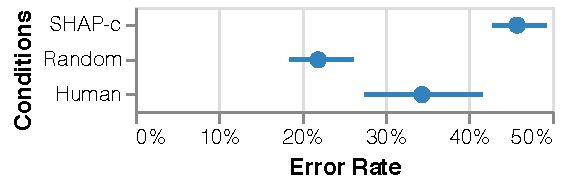
\includegraphics[width=1\columnwidth]{figures/err_rate.pdf}
\vspace{-15pt}
\caption{
Error rates on counterfactuals in different conditions. The higher the error rate, the more information missed by the participants, therefore can better complement manual counterfactual analysis and SHAP.
}
\vspace{-10pt}
\label{fig:err_rate}
\end{figure}
\end{comment}

\paragraph{Results.}
As a within-subject study, we compared the error rate of human simulations across the three conditions.
Participants only did slightly better than random guess on \cshap cases, with error rate $e=45\%\pm6\%$.
If presented, these counterfactuals should bring more insights than hiring an expert graduate student to create counterfactuals ($e=39\%\pm11\%$), and more effectively: each graduate student had to spend 1.5--2 hours to generate 20 ``abnormal'' counterfactuals. 
\crandom cases can be easily simulated ($e=23\%\pm6\%$), indicating the importance of abnormal counterfactuals.

Another graduate student rated the fluency of counterfactuals, and verified that the simulation failure was not due to nonsensical noise.
Interestingly, the rater deemed more than 95\% counterfactuals to be likely written by native speakers in both \sysname conditions, but only 85\% for \chuman, indicating that humans wrote ungrammatical sentences in order to find puzzling behavior.

Participants' manual analysis revealed that they mostly erred when they missed the inspection spot.
They focused mostly on what SHAP explanations deemed important, and ignored what was unimportant --- 84\% of their querying counterfactuals perturbed the most important features in the instance.\footnote{Tokens with weights higher than the 85\% quantile of all the weights in the instance.}
For example, they repeatedly perturbed ``depression'' in Figure~\ref{fig:explanation}A, and therefore had to guess when simulating Figure~\ref{fig:explanation}B.
In their survey responses, 7 participants explicitly stated their focus on important features, confirming that feature attributions can lead to incomplete comprehension.

There are also 24\% of the missed \cshap cases where participants only partially inspected the related pattern,\footnote{At least one of their queries perturbed the same spans as $\xp$, and query text overlaps with the $\xp$ for over 70\%.} and were misled by it --- ``followed similar examples I tried,'' as one subject articulated.
They could not to imagine the model predicting \emph{Duplicate} on Figure~\ref{fig:explanation}B (\swap{help}{find}), when it predicted \emph{Non-Duplicate} on their query \exinline{How do I \swap{help}{play with}...?}
The number dropped to $15\%$ for the \chuman condition, showing that \cshap found more bugs in spots that participants considered inspected.

\subsection{Discussions}

\sysname counterfactuals is preferable over hiring a second expert analyst: they help find more insights at lower annotation cost, with less ungrammatical changes, and help extend manual inspection more exhaustively.
However, certain forms of explanation selection is necessary to overcome the obvious ones. 
The abnormality is one useful criteria that aligns with humans' cognitive processes, but humans should also be able to drive the selection, and acquire concrete foils for any spans \emph{they} do not understand.
For example, an analyst can \texttt{BLANK} ``friend'' in Q2 in Figure~\ref{fig:explanation}C, and observe the model's unstable behavior: it predicts \emph{Non-duplicate} when \remove{friend} is changed to \add{woman}, \add{professional}, but remains \emph{Duplicate} at \add{man}, \add{student}.
We discuss the interactions in \S\ref{sec:err_analysis}.

As \citet{miller} noted, individual users should require less explanation the more they interact with a system.
The fact that \sysname can still complement users' mental models, even after they see the feature attributions and manually inspect the model, indicates that the gain can be more prominent when such explanation and model access is not available. 
We envision that the abnormality selection can also help select standalone explanations, if the expectation is instead estimated without feature attribution explanations (\eg he distance in the latent space~\cite{reimers-2019-sentence-bert}).
We defer the exploration to future work.













%%%%%%%%%%%%%%%%%%%%%%%%%%%%%%%%%%%%%%%%%%%%%%%%%%%%%%%%%%%%%%%%%%%%%%%%%%%%%%%%


%\wts{Finding bugs missed by the feature attribution, and concretizing the opaque weights using readable examples.}
\subsection{Selection: Abnormalities as Explanations}
\label{subsec:local_explain}

\footnotetext{From BERT \qqp model: \url{https://huggingface.co/textattack/bert-base-uncased-QQP}}

Counterfactual explanations have been elusive in NLP, despite being more intuitive than feature attribution methods~\cite{miller}.
Compared to the opaque feature weights in Figure~\ref{fig:explanation}A, Figure~\ref{fig:explanation}B more intuitively shows that the BERT \qqp model considers \remove{help} trivial: 
changing it to \add{find} does not change the prediction.
Meanwhile, the concrete counterfactuals can be overwhelming, and therefore are less suitable for providing overviews.
Here, we combine the benefits of the two methods, by \emph{augmenting} feature attribution methods (\eg SHAP~\cite{NIPS2017_7062} or LIME~\cite{Ribeiro2016WhySI}) with \emph{abnormal} counterfactuals, which are observed to be more salient~\cite{miller}.

Given a model $f$, the relationship $\relation{\xp}$ we use for capturing abnormality is the disagreement (distance) between \emph{the actual change of model prediction $\dist(\xp, x)$, and the expected change $\E[\dist(\xp, x)]$}:
$$\Delta\dist(\xp, x) = \dist(\xp, x)-\E[\dist(\xp, x)]$$

We quantify $\dist(\xp, x)$ based on the the prediction probability of $f$ on $x$ and $\xp$.
$\E[\dist(\xp, x)]$ is defined as the estimated importance (SHAP weights) of the perturbed tokens in $x$ (details in Appendix~\ref{appendix:exp_rank}).
We select two \emph{expectation violation} counterfactuals: %according to $\Delta\dist(\xp, x)$.
(1) \emph{unexpected prediction flipping}, when the perturbation is trivial ($\argmax_{\xp} \Delta\dist(\xp, x)$).
In Figure~\ref{fig:explanation}C, \swap{friend}{woman} changes the prediction from \emph{Duplicate} to \emph{Non-Duplicate}, even though ``friend'' has low weight.
(2) \emph{unexpected prediction preserving}, when the perturbation is aggressive. ($\argmax_{\xp} -\Delta\dist(\xp, x)$).
In Figure~\ref{fig:explanation}D, changing the important \remove{in depression} still results in \emph{Duplicate}.

The abnormal $\xp$ additionally highlights an often overlooked nuance: feature attribution methods estimate weights by \emph{masking} words, and therefore may not reflect models' reactions to substitutions or additions.
Used together, we expect them to more comprehensively present the predictor.

The abnormality selection can also be generalized beyond feature attribution.
We can select standalone explanations, if we instead use the distance in the latent space~\cite{reimers-2019-sentence-bert} as $\E[\boldsymbol{\cdot}]$.
We defer the exploration to future work.


\subsection{Experiment: Counterfactual Simulation}
\label{subsec:exp_user_study}

To verify whether our counterfactual explanations can complement SHAP, we conduct a user study on counterfactual simulation~\cite{hase2020evaluating}, \ie participants predict a model's behavior on $\xp$.
Intuitively, the more they simulate incorrectly, the more information they grasp \emph{if we show the $\xp$}.

%We conduct a user study to verify whether our counterfactual explanations can complement SHAP.
%, as the setup nicely combines the overview provided by SHAP, and the decision boundaries it omits.
%\footnote{We defer more sophisticated designs and evaluations for interactive and global explanation to future work.}
%, where participants are asked to predict model's behavior on the given variations of a base example.
%The study takes the form of counterfactual simulation~\cite{hase2020evaluating}, with participants predicting a model's behavior on $\xp$.
%Intuitively, the more they simulate incorrectly, the more information they grasp \emph{if we show the counterfactuals}.

\paragraph{Procedure.}
We recruited 13 graduate students with experience in model explanations, and asked them to simulate the aforementioned \qqp model for 20 rounds.
In each round, the participants were given a base example, model prediction on it, and the SHAP weights, displayed as in Figure~\ref{fig:explanation}A.
Moreover, they could create up to 10 counterfactuals on their own, and query the model predictions on them (they used around 6 chances.)
%More interactions with the predictor usually result in better mental models~\cite{miller}, and we are interested in whether our counterfactuals \emph{still add information} after sufficient interactions (they usually used 6 chances.)
Participants then simulated the model predictions on six counterfactuals, two from each of the following three conditions.
We concluded the study with surveys on their model inspection and simulation strategies.
%The interface is in Appendix~\ref{appendix:exp_user_study}.

%We validate this hypothesis in user study, where expert users did slightly better than random (accuracy: $55 \pm 6\%$) at predicting what a model would do on \sysname counterfactuals, even after seeing SHAP explanations \cite{NIPS2017_7062} and manually creating counterfactuals to explore the model's behavior. This indicates that seeing such explanations would add a lot of information that users are currently missing (much of which consisting of mistaken model predictions) even if when they perform manual counterfactual analysis and use feature attribution methods.


\newcommand{\cshap}{\emph{SHAP-c}\xspace}
\newcommand{\crandom}{\emph{Random}\xspace}
\newcommand{\chuman}{\emph{Human}\xspace}
\paragraph{Conditions.} 
We compare three types of counterfactuals:
(1) \cshap, the \sysname-generated, abnormal counterfactuals, selected to complement SHAP; 
(2) \crandom, the randomly selected \sysname counterfactuals; 
(3) \chuman, the human-generated counterfactuals, in which two graduate students (not participants) played with the model, and each created one $\xp$ where the prediction was incorrect and counterintuitive according to the SHAP score on $x$.
The authors manually checked that all counterfactuals were fluent and unambiguous.

% \begin{comment}
\begin{figure}[t]
\centering
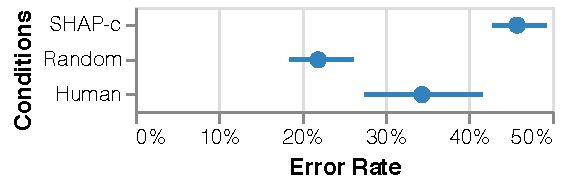
\includegraphics[width=1\columnwidth]{figures/err_rate.pdf}
\vspace{-15pt}
\caption{
Error rates on counterfactuals in different conditions. The higher the error rate, the more information missed by the participants, therefore can better complement manual counterfactual analysis and SHAP.
}
\vspace{-10pt}
\label{fig:err_rate}
\end{figure}
% \end{comment}

\paragraph{Results.}
As a within-subject study, we compared \emph{the error rate of human simulations across the three conditions}.
%As in Figure~\ref{fig:err_rate}, 
Participants were able to simulate the cases in \crandom (error rate $e=23\%\pm6\%$), possibly because they are are aligned with participants' mental models built on SHAP explanations and their interactions with the model~\cite{miller}.
They missed more \chuman ($e=39\%\pm11\%$) cases, and were even worse on \cshap ($45\%\pm 6\%$, only slightly better than random guess).
%, though the confidence intervals overlap.
This result shows that \cshap counterfactuals provide insight beyond feature attributions and manual counterfactual analysis, and \emph{would still add value if they were presented.}
They are also at least as effective as the \chuman examples, which are very expensive to create: each graduate student spent 1.5--2 hours to generate 20 ``abnormal'' counterfactuals.

Usually, participants simulated the model incorrectly because they missed certain inspection spots.
For example, they repeatedly perturbed ``depression'' in Figure~\ref{fig:explanation}A, and therefore had to guess when simulating Figure~\ref{fig:explanation}B.
However, in 24\% of the missed \cshap cases, participants successfully inspected the related pattern,\footnote{At least one of their queries perturbed the same spans as $\xp$, and query text overlaps with the $\xp$ for over 70\%.} but were misled by it --- ``followed similar examples I tried,'' as one subject articulated.
It was hard for them to imagine the model predicting \emph{Duplicate} on Figure~\ref{fig:explanation}B (\swap{help}{find}), when it predicted \emph{Non-Duplicate} on their query \exinline{How do I \swap{help}{play with}...?}
The number dropped to $15\%$ for the \chuman condition.
In other words, \emph{\cshap found more bugs in spots that participants considered inspected.}
%\hao{this is very interesting. close by summarizing the conclusion?}


\paragraph{Takeaways.}
\sysname counterfactuals complement feature attribution methods as effectively as hiring a second expert for the analysis (but much cheaper).
In particular, they highlight errors where humans may be misled by their own analysis.
